\documentclass{standalone}
\usepackage{tikz}
\usepackage{bm}
\begin{document}
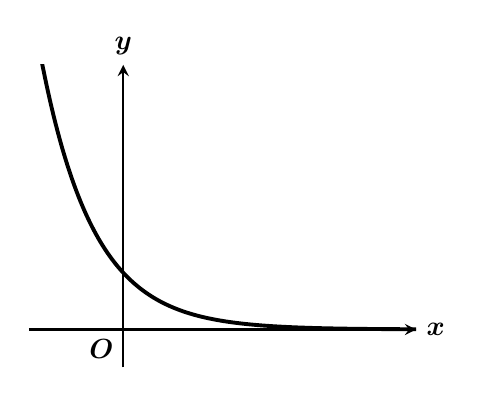
\begin{tikzpicture}[>=stealth, scale=0.6, font=\bfseries]
  % From unit2a/6-D.png: y = 1.2e^(-0.9x); exponential decay
  \draw[->, thick] (-2.0,0) -- (6.2,0) node[right] {$\bm{x}$};
  \draw[->, thick] (0,-0.8) -- (0,5.6) node[above] {$\bm{y}$};
  \node[below left] at (0,0) {$\bm{O}$};
  \begin{scope}
    \clip (-2.0,-0.8) rectangle (6.2,5.6);
    \draw[line width=1.4pt, smooth, samples=150, domain=-2.0:6.2] plot (\x, {1.2*exp(-0.9*\x)});
  \end{scope}
\end{tikzpicture}
\end{document}
